\documentclass[pdf,10pt]{beamer}
\mode<presentation>{\usetheme{Madrid}}

%List of packages
\usepackage{algpseudocode}
\usepackage{algorithm}

\renewcommand{\algorithmicrequire}{\textbf{Input:}}
\renewcommand{\algorithmicensure}{\textbf{Initialize:}}
%\usepackage{amsmath}
\usepackage{hyperref}
\usepackage{cleveref}

\def\R{\mathbb{R}}


% \useoutertheme{infolines}
%%%%%%%%%%%%%%%%%%%%%%%%%%%%%% Metadata %%%%%%%%%%%%%%%%%%%%%%%%%%%%%%
% \hypersetup
% {
% 	%Separate multiple authors by comma
% 	pdfauthor={Dmitry Beresnev, Vsevolod Klyushev},
% 	pdftitle={HDDA: Recommendation System Project},
% 	pdfsubject={Instructions, Tutorials, Guidelines},
% 	pdfkeywords={SPSAS19, guidelines, presentation format},
% 	colorlinks=false
% }

%%%%%%%%%%%%%%%%%%%%%%%%%%%%%% Title related %%%%%%%%%%%%%%%%%%%%%%%%%%%%%%
\setbeamertemplate{subsection in toc}[default]

%The contact for one of the authors MUST be embedded on the title (see below)
\title[]{HDDA Recommendation systems
via approximate matrix factorization}
% Subtitle (if needed)
% \subtitle{Team 1}
%For LICENSE, we suggest CC-BY-SA, but you are free to choose your own as long
%as the LICENSE you choose is AT LEAST as permissive as CC-BY-SA
\date[2024]{Innopolis University --- IU --- 2024\\ \vspace{0.5cm}}
\author[Beresnev, Klyushev \hspace{0.2cm}]{\texorpdfstring{Dmitry Beresnev \\ Vsevolod Klyushev}{}}


%%%%%%%%%%%%%%%%%%%%%%%%% Presentation begins here %%%%%%%%%%%%%%%%%%%%%%%%%
\begin{document}


\begin{frame}
  \titlepage
\end{frame}

\begin{section}{Introduction}

 \begin{subsection}{Problem formulation}

   \begin{frame}
     \frametitle{Initial problem}

     We need to solve the following problem:
     \begin{equation} \label{initial}
       \min_{U \in \R^{m\times r}, V \in \R^{r\times n}} \|W \circ (X - UV)\|^2_F
     \end{equation}
     where:
     \begin{itemize}
       \item $X$ --- target matrix ($m\times n$);
       \item $W$ --- binary mask;
       \item $r$ --- rank of factorization;
     \end{itemize}

   \end{frame}

   \begin{frame}
     \frametitle{Gradients}

     In order to use gradient methods, we need to derive it with respect to each parameter ($U$ and $V$) (full derivation might be found \href{https://hushtheblock.github.io/2020/08/06/Derivative-of-a-function/}{\underline{here}}):
     \begin{equation}
       \cfrac{\partial \|W \circ (X - UV)\|^2_F}{\partial U} = -2 (W \circ X) V^T + 2 (W \circ (UV)) V^T
     \end{equation}

     \begin{equation}
       \cfrac{\partial \|W \circ (X - UV)\|^2_F}{\partial V} = -2 U^T (W \circ X) + 2 U^T (W \circ (UV))
     \end{equation}


   \end{frame}

   \begin{frame}

     \frametitle{Improved problem}

     As a modified problem, we decided just to add some regularization. This brings us to the following forms:

     \begin{equation}
       \min_{U \in \R^{m*r}, V \in \R^{r*n}} \|W \circ (X - UV)\|^2_F + \lambda\|U\|^2_F + \lambda\|V\|^2_F
     \end{equation}

     \begin{equation}
       \cfrac{\partial (\|W \circ (X - UV)\|^2_F + \lambda\|U\|^2_F + \lambda\|V\|^2_F)}{\partial U} = -2 (W \circ X) V^T + 2 (W \circ (UV)) V^T + 2\lambda U
     \end{equation}

     \begin{equation}
       \cfrac{\partial (\|W \circ (X - UV)\|^2_F + \lambda\|U\|^2_F + \lambda\|V\|^2_F)}{\partial V} = -2 U^T (W \circ X) + 2 U^T (W \circ (UV)) + 2\lambda V
     \end{equation}

     where $\lambda$ --- regularization parameter

   \end{frame}

 \end{subsection}
\end{section}


\begin{section}{LR Strategies}

 \begin{frame}
   \frametitle{Constant + decreasing}

   We can take constant step, or such step, that would decrease with increase of iterations. For example, $\gamma = \frac{1}{\sqrt{k}}$, where $k$ --- number of iterations.
 \end{frame}


 \begin{frame}
   \frametitle{Estimate $1/L$}
   \begin{algorithm}[H]
     \caption{Estimate $1/L$}\label{algo:lr_est}
     \begin{algorithmic}[0]
       \Require{$\theta$ (point), $\nabla f(\theta)$ (gradient function), $p$ (desired direction), $\beta$ (multiplier), $t$ (max iterations) }

       \State{$\alpha \gets 1 $}
       \For{$i = 1$ \textbf{to} $t$}
       \State{$\theta_i \gets \theta + \alpha p $}
       \If{$\|\nabla f(\theta) -\nabla f(\theta_i)\| > \frac{1}{\alpha} \|\theta -  \theta_i\|$}
       \State{$\alpha \gets \beta \cdot \alpha$ }
       \If{$\alpha < \epsilon$}
       \State{\Return{$\alpha$}}
       \EndIf{}
       \Else{}
       \State{\Return{$\alpha$}}
       \EndIf{}
       \EndFor{}
       \State{\Return{$\alpha$}}

     \end{algorithmic}
   \end{algorithm}
 \end{frame}


 \begin{frame}
   \frametitle{Armijo}
   \begin{figure}[hbt]
     \centering
     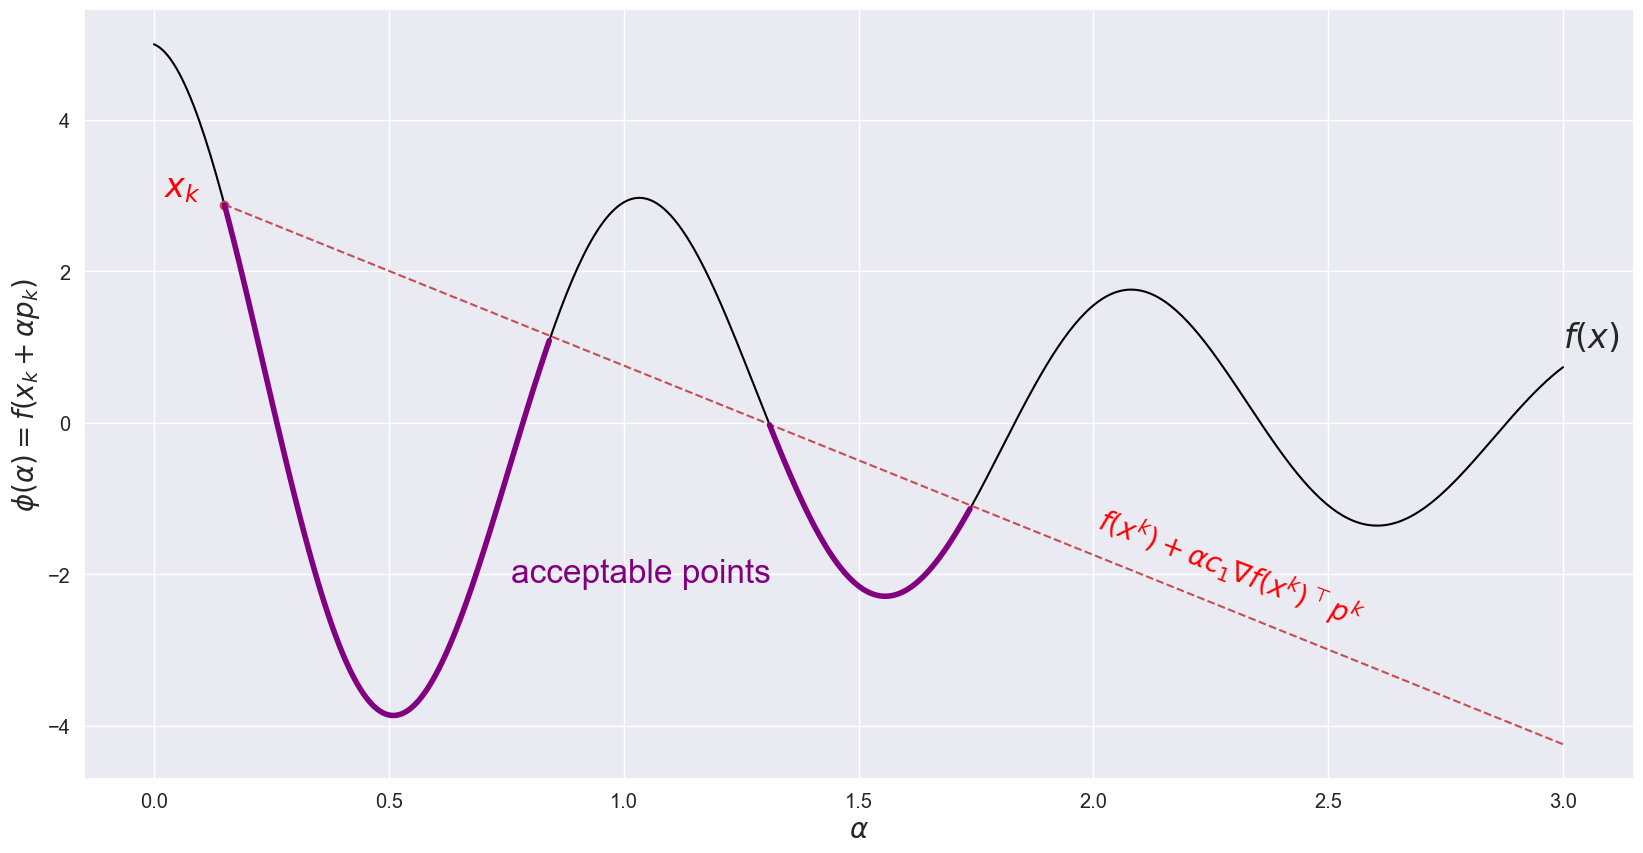
\includegraphics[width=\textwidth,keepaspectratio]{../data/armijo.png}
     \caption[Armijo rule]{Armijo rule}\label{fig:armijo}
   \end{figure}
 \end{frame}


 \begin{frame}

   \begin{algorithm}[H]
     \frametitle{Armijo}
     \caption{Armijo Step}\label{algo:lr_armijo}
     \begin{algorithmic}[0]
       \Require{$\theta$ (point), $f(\theta)$ (objective function), $p$ (desired direction), $\beta$ (multiplier), $c_1 > 0$, $t$ (max iterations) }

       \State{$\alpha \gets 1 $}
       \For{$i = 1$ \textbf{to} $t$}
       \State{$\theta_i \gets \theta + \alpha p $}
       \If{$f(\theta_i) > f(\theta) + c_1 \alpha \langle \nabla_{\theta} f(\theta), p \rangle $}
       \State{$\alpha \gets \beta \cdot \alpha$ }
       \If{$\alpha < \epsilon$}
       \State{\Return{$\alpha$}}
       \EndIf{}
       \Else{}
       \State{\Return{$\alpha$}}
       \EndIf{}
       \EndFor{}
       \State{\Return{$\alpha$}}

     \end{algorithmic}
   \end{algorithm}
 \end{frame}




 \begin{frame}
   \frametitle{Curvature condition}
   \begin{figure}[hbt]
     \centering
     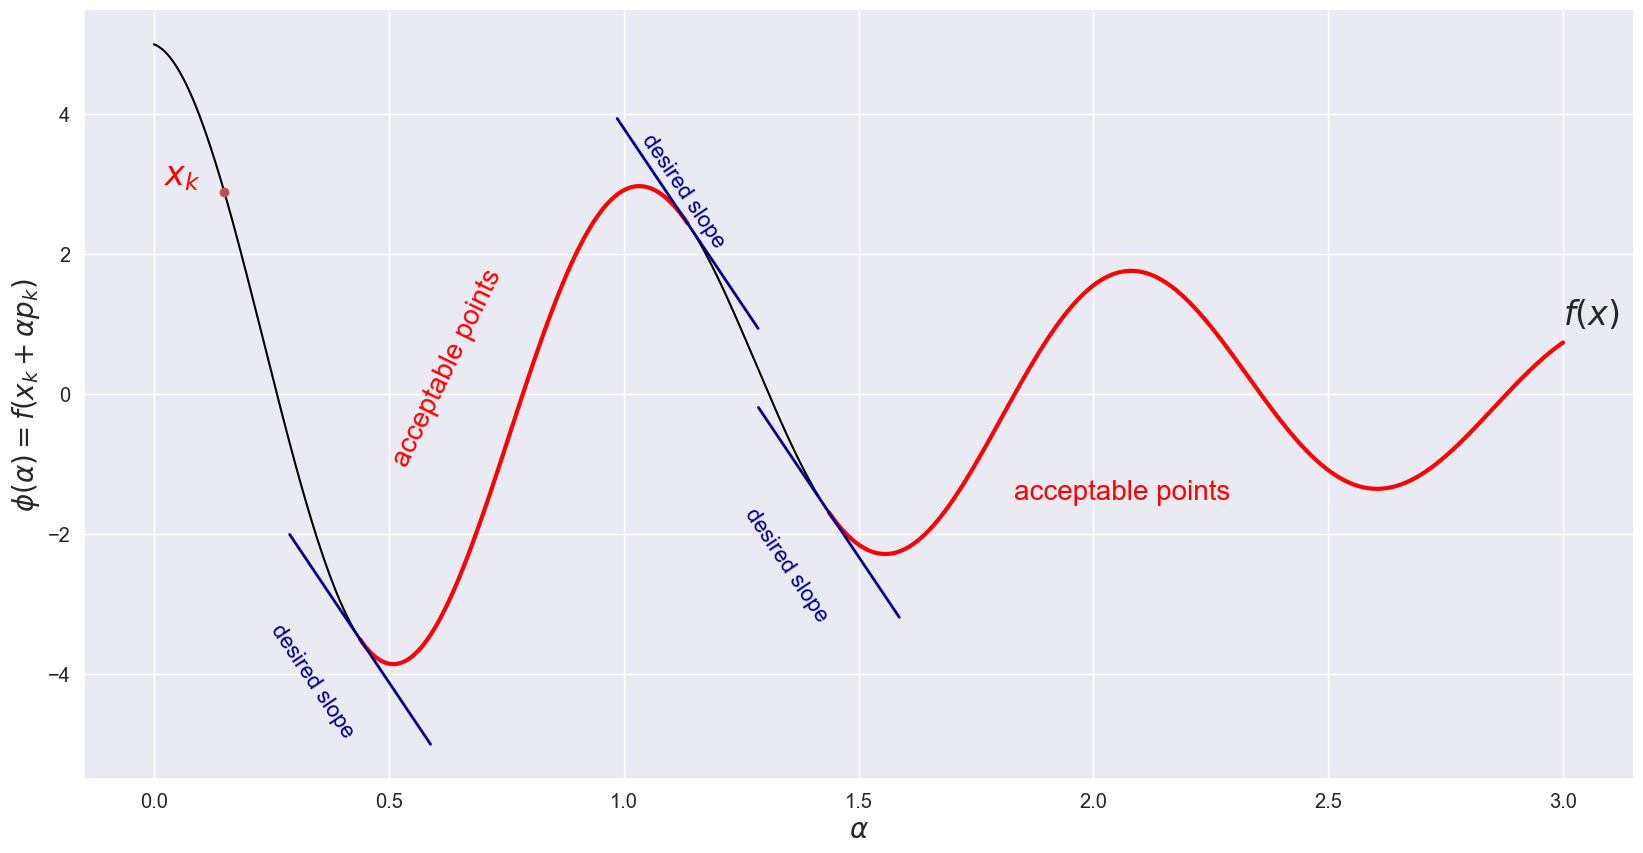
\includegraphics[width=\textwidth,keepaspectratio]{../data/curvature.png}
     \caption[Curvature condition]{Curvature condition}\label{fig:curvature}
   \end{figure}
 \end{frame}



 \begin{frame}
   \frametitle{Bisection Weak Wolfe}
   \begin{figure}[H]
     \centering
     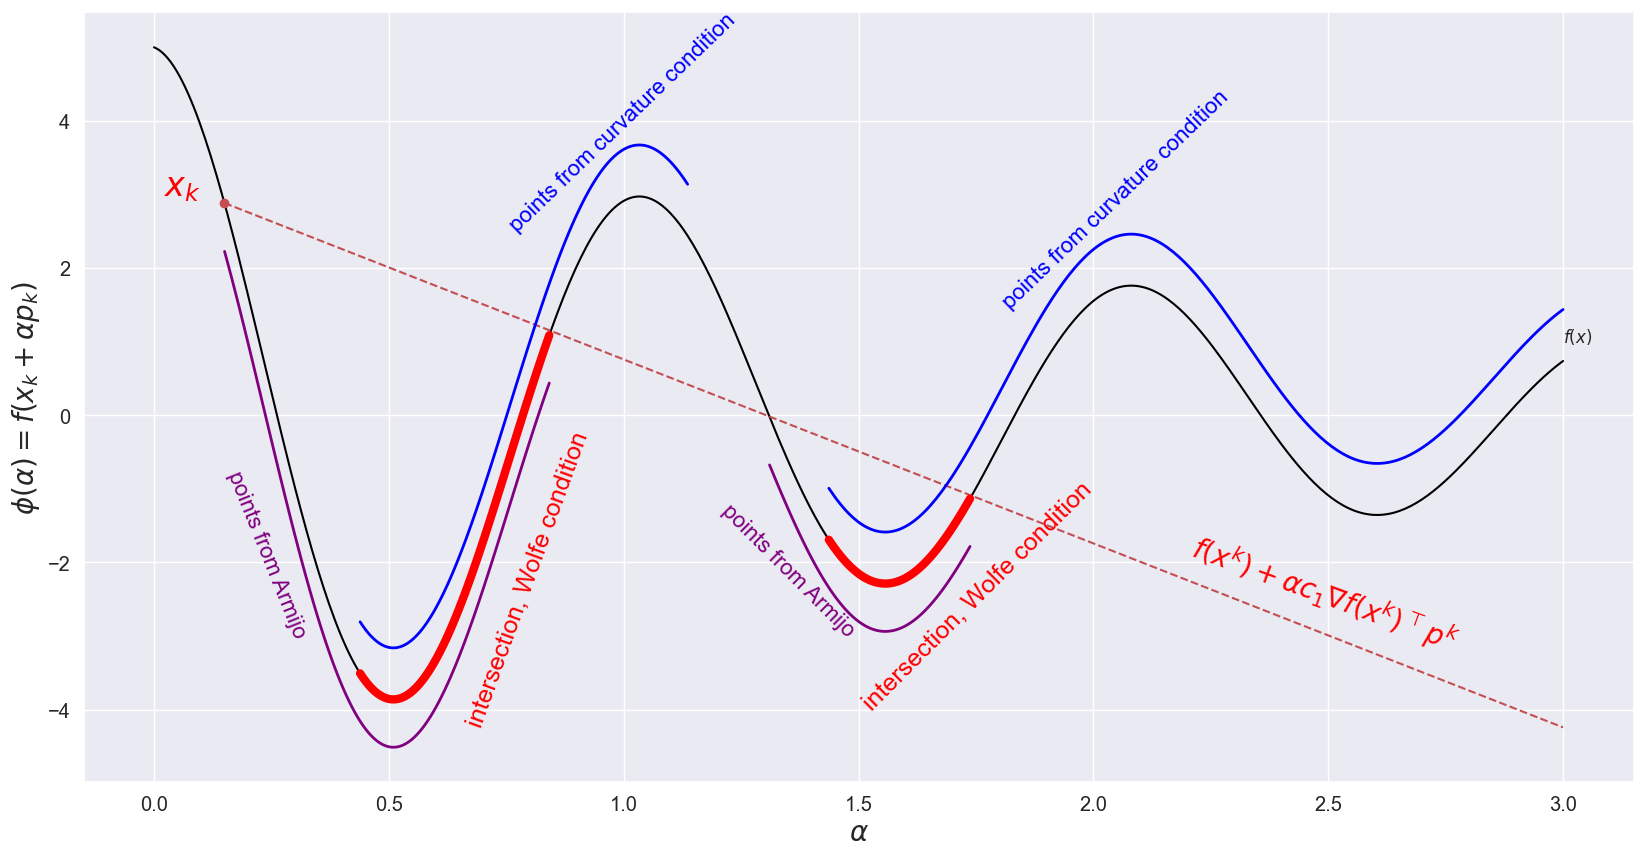
\includegraphics[width=\textwidth,keepaspectratio]{../data/weak_wolfe.png}
     \caption[Weak Wolfe conditions]{Weak Wolfe conditions}\label{fig:weak_wolfe}
   \end{figure}
 \end{frame}

 \begin{frame}
   \frametitle{Bisection Weak Wolfe}
   \begin{algorithm}[H]
     \tiny
     \caption{Bisection Weak Wolfe Step}\label{algo:lr_biwolfe}
     \begin{algorithmic}[0]
       \Require{$\theta$ (point), $f(\theta)$ (objective function), $p$ (desired direction), $\beta$ (multiplier), $c_1>0$, $c_2 >c_1$, $t$ (max iterations) }

       \State{$\alpha \gets 1 $}
       \State{$a \gets 0 $}  \Comment{Lower bound}
       \State{$b \gets +\infty $}  \Comment{Upper bound}
       \For{$i = 1$ \textbf{to} $t$}
       \State{$\theta_i \gets \theta + \alpha p $}

       \If{$f(\theta_i) > f(\theta) + c_1 \alpha \langle \nabla_{\theta} f(\theta), p \rangle$} \Comment{Armijo condition}

       \State{$b \gets \alpha$ }
       \State{$\alpha \gets \frac{1}{2} (a+b)$ } \Comment{Decrease step}

       \ElsIf{$\langle p, \nabla_{\theta}f(\theta_i)  \rangle < c_2  \langle p, \nabla_{\theta}f(\theta)  \rangle $} \Comment{Curvature condition}
       \State{$a \gets \alpha$ }

       \If{$b= +\infty$}
       \State{$\alpha \gets 2a$}
       \Else{}
       \State{$\alpha \gets \frac{1}{2} (a+b)$ } \Comment{Increase step}
       \EndIf{}
       \Else{}
       \State{\Return{$\alpha$}}
       \EndIf{}
       \EndFor{}
       \State{\Return{$\alpha$}}

     \end{algorithmic}
   \end{algorithm}
 \end{frame}

 \begin{frame}
   \frametitle{Strong Wolfe}
   \begin{figure}[H]
     \centering
     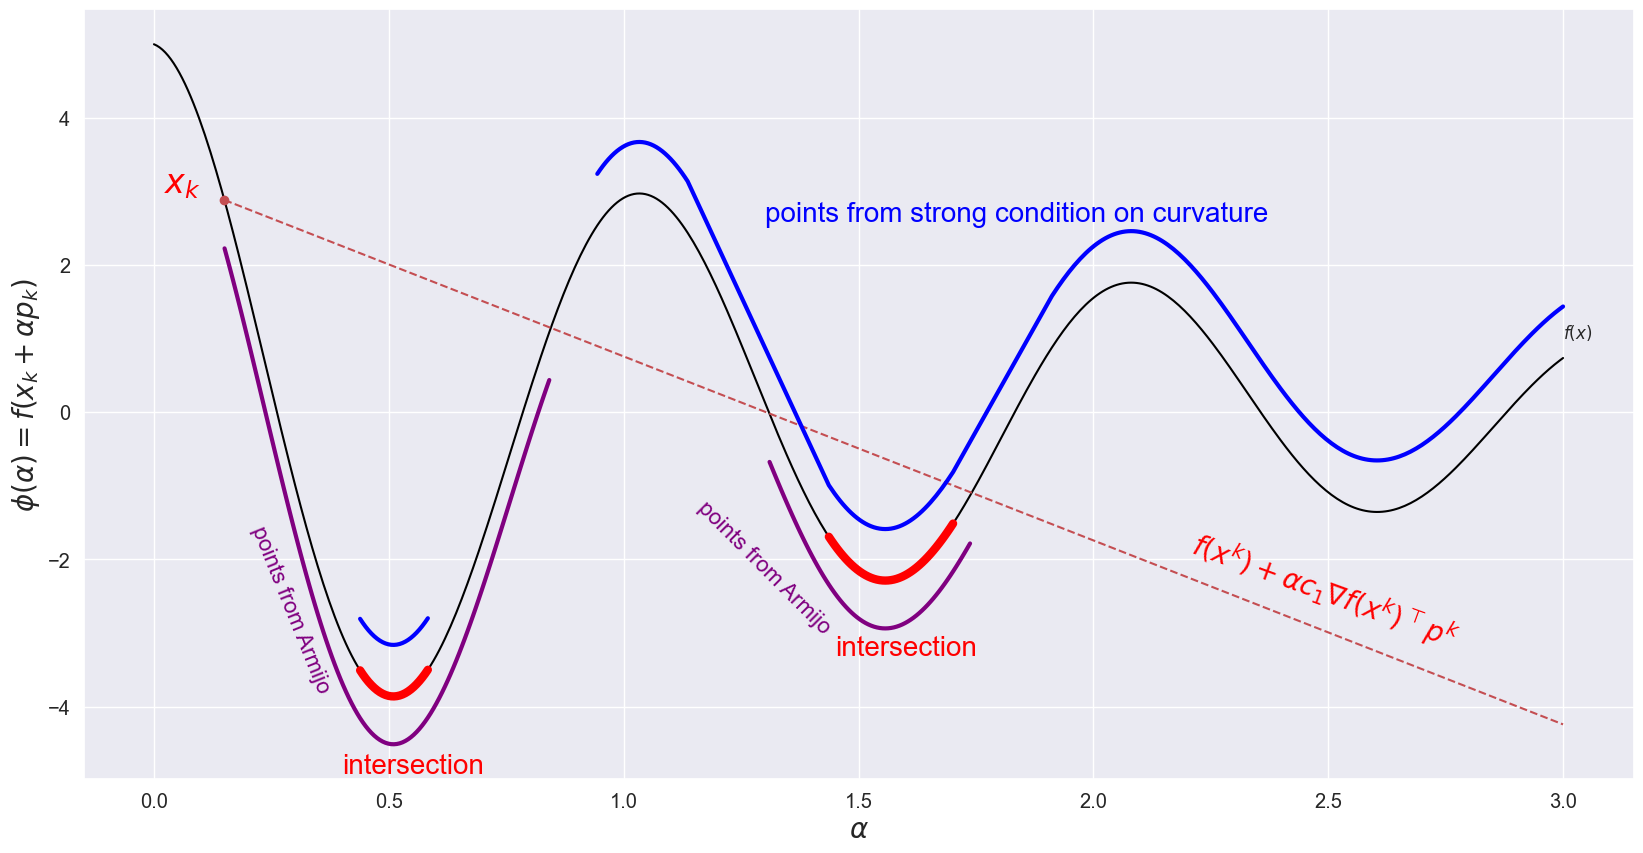
\includegraphics[width=\textwidth,keepaspectratio]{../data/strong_wolfe.png}
     \caption[Strong Wolfe conditions]{Strong Wolfe conditions}\label{fig:strong_wolfe}
   \end{figure}
 \end{frame}

 \begin{frame}
   \frametitle{Strong Wolfe}
   \begin{algorithm}[H]
     \caption{Strong Wolfe Step}\label{algo:lr_wolfe}
     \begin{algorithmic}[0]
       % \tiny
       \Require{$\theta$ (point), $f(\theta)$ (objective function), $p$ (desired direction), $\beta$ (multiplier), $c_1>0$, $c_2 >c_1$, $t$ (max iterations) }

       \State{$\alpha \gets 1 $}
       \For{$i = 1$ \textbf{to} $t$}
       \State{$\theta_i \gets \theta + \alpha p $}
       \If{$\bigl(f(\theta_i) > f(\theta) + c_1 \alpha \langle \nabla_{\theta} f(\theta), p \rangle \bigr)$
         \textbf{or} $\bigl( \| \langle p, \nabla_{\theta}f(\theta_i)  \rangle  \| > c_2 \| \langle p, \nabla_{\theta}f(\theta)  \rangle \|  \bigr)$}
       \State{$\alpha \gets \beta \cdot \alpha$ }
       \If{$\alpha < \epsilon$}
       \State{\Return{$\alpha$}}
       \EndIf{}
       \Else{}
       \State{\Return{$\alpha$}}
       \EndIf{}
       \EndFor{}
       \State{\Return{$\alpha$}}

     \end{algorithmic}
   \end{algorithm}
 \end{frame}





\end{section}

\begin{section}{Optimizers}

 \begin{frame}
   \frametitle{Gradient Descent}

   \begin{algorithm}[H]
     \caption{Gradient Descent optimizer}\label{algo:gd}
     \begin{algorithmic}[0]
       \Require{$\theta_0$ (parameters to optimize), $f(\theta)$ (objective function), $\mathcal{L}(p)$ (step size choosing strategy) }

       \For{$t = 1$ \textbf{to} $\dots$}
       \State{$p_t \gets -\nabla_{\theta}f_t(\theta_{t-1}) $} \Comment{Step direction}
       \State{Choose step size $\gamma$ according to $\mathcal{L}(p_t)$}
       \State{$\theta_t \gets \theta_{t-1} + \gamma p_t $}
       \EndFor{}

       \State{\Return{$\theta_t$}}

     \end{algorithmic}
   \end{algorithm}

 \end{frame}

 \begin{frame}
   \frametitle{Adaptive Gradient Descent}
   \begin{algorithm}[H]
     \caption{Adaptive Gradient Descent}\label{algo:lr_adaptive}
     \begin{algorithmic}[0]
       \Require{$x_0$ (parameters to optimize), $f(x)$ (objective function) }
       \Ensure{$\lambda_0 > 0$ (small start step), $\theta_0 \gets +\infty$ }

       \State{$x_1 \gets x_0 - \lambda_0 \nabla f(x_0)$}
       \For{$t = 1$ \textbf{to} $\ldots$}
       \State{$\lambda_t = \min\Bigl\{
         \sqrt{1+\theta_{t-1}}\lambda_{t-1},\frac{\|x_{t}-x_{t-1}\|}{2\|\nabla
         f(x_{t})-\nabla f(x_{t-1})\|}\Bigr\}$}
       \State{$x_{t+1} \gets x_t - \lambda_t \nabla f(x_t)$}
       \State{$\theta_t \gets \frac{\lambda_t}{\lambda_{t-1}}$}
       \EndFor{}
       \State{\Return{$x_t$}}
     \end{algorithmic}
   \end{algorithm}
 \end{frame}


 \begin{frame}
   \frametitle{Heavy Ball}
   \begin{algorithm}[H]
     % \tiny
     \caption{Heavy Ball optimizer}\label{algo:hb}
     \begin{algorithmic}[0]
       \Require{$\theta_0$ (parameters to optimize), $f(\theta)$ (objective function), $\beta$ (momentum), $\mathcal{L}(p)$ (step size choosing strategy) }

       \For{$t = 1$ \textbf{to} $\dots$}
       \State{$g_t \gets \nabla_{\theta}f_t(\theta_{t-1}) $}

       \If{$\beta \neq 0$}
       \If{$t > 1$}
       \State{$b_t \gets \beta b_{t-1} + g_t$}
       \Else{}
       \State{$b_t \gets g_t$}
       \EndIf{}
       \State{$g_t \gets b_t$}
       \EndIf{}

       \State{$p_t \gets -g_t $} \Comment{Step direction}
       \State{Choose step size $\gamma$ according to $\mathcal{L}(p_t)$}
       \State{$\theta_t \gets \theta_{t-1} + \gamma p_t $}
       \EndFor{}

       \State{\Return{$\theta_t$}}

     \end{algorithmic}
   \end{algorithm}

 \end{frame}

 \begin{frame}
   \frametitle{Nesterov}
   \begin{algorithm}[H]
     % \tiny
     \caption{Nesterov optimizer}\label{algo:nesterov}
     \begin{algorithmic}[0]
       \Require{$\theta_0$ (parameters to optimize), $f(\theta)$ (objective function), $\beta$ (momentum), $\mathcal{L}(p)$ (step size choosing strategy) }

       \For{$t = 1$ \textbf{to} $\dots$}
       \State{$g_t \gets \nabla_{\theta}f_t(\theta_{t-1}) $}

       \If{$\beta \neq 0$}
       \If{$t > 1$}
       \State{$b_t \gets \beta b_{t-1} + g_t$}
       \Else{}
       \State{$b_t \gets g_t$}
       \EndIf{}
       \State{$g_t \gets g_t + \beta b_t$}
       \EndIf{}

       \State{$p_t \gets -g_t $} \Comment{Step direction}
       \State{Choose step size $\gamma$ according to $\mathcal{L}(p_t)$}
       \State{$\theta_t \gets \theta_{t-1} + \gamma p_t $}
       \EndFor{}

       \State{\Return{$\theta_t$}}

     \end{algorithmic}
   \end{algorithm}
 \end{frame}

 \begin{frame}
   \frametitle{AdaGrad}
   \begin{algorithm}[H]
     \caption{AdaGrad optimizer}\label{algo:adagrad}
     \begin{algorithmic}[0]
       \Require{$\theta_0$ (parameters to optimize), $f(\theta)$ (objective function), $\mathcal{L}(p)$ (step size choosing strategy) }
       \Ensure{$s_0 \gets 0$ (cumulative square sum)}

       \For{$t = 1$ \textbf{to} $\dots$}
       \State{$g_t \gets \nabla_{\theta}f_t(\theta_{t-1}) $}
       \State{$s_t \gets \alpha s_{t-1} + g_t^2 $}
       \State{$p_t \gets -g_t / (\sqrt{s_t} + \epsilon) $} \Comment{Step direction}

       \State{Choose step size $\gamma$ according to $\mathcal{L}(p_t)$}
       \State{$\theta_t \gets \theta_{t-1} + \gamma p_t $}
       \EndFor{}

       \State{\Return{$\theta_t$}}

     \end{algorithmic}
   \end{algorithm}

 \end{frame}

 \begin{frame}
   \frametitle{RMSProp}
   \begin{algorithm}[H]
     \caption{RMSProp optimizer}\label{algo:rmsprop}
     \begin{algorithmic}[0]
       \Require{$\theta_0$ (parameters to optimize), $f(\theta)$ (objective function), $\alpha$ (alpha), $\mathcal{L}(p)$ (step size choosing strategy) }
       \Ensure{$v_0 \gets 0$ (square average)}

       \For{$t = 1$ \textbf{to} $\dots$}
       \State{$g_t \gets \nabla_{\theta}f_t(\theta_{t-1}) $}
       \State{$v_t \gets \alpha v_{t-1} + (1-\alpha) g_t^2 $}
       \State{$p_t \gets -g_t / (\sqrt{v_t} + \epsilon) $} \Comment{Step direction}

       \State{Choose step size $\gamma$ according to $\mathcal{L}(p_t)$}
       \State{$\theta_t \gets \theta_{t-1} + \gamma p_t $}
       \EndFor{}

       \State{\Return{$\theta_t$}}

     \end{algorithmic}
   \end{algorithm}
 \end{frame}

 \begin{frame}
   \frametitle{Adam}
   \begin{algorithm}[H]
     \caption{Adam optimizer}\label{algo:adam}
     \begin{algorithmic}[0]
       \Require{$\theta_0$ (parameters to optimize), $f(\theta)$ (objective function), $\beta_1$, $\beta_2$ (alpha), $\mathcal{L}(p)$ (step size choosing strategy) }
       \Ensure{$m_0 \gets 0$ (first moment), $v_0 \gets 0$ (second moment)}

       \For{$t = 1$ \textbf{to} $\dots$}
       \State{$g_t \gets \nabla_{\theta}f_t(\theta_{t-1}) $}
       \State{$m_t \gets \beta_1 m_{t-1} + (1-\beta_1) g_t $}
       \State{$v_t \gets \beta_2 v_{t-1} + (1-\beta_2) g_t^2 $}

       \State{$\hat{m_t} \gets m_t / (1- \beta_1^t) $}
       \State{$\hat{v_t} \gets v_t / (1- \beta_2^t) $}

       \State{$p_t \gets -\hat{m_t} / (\sqrt{\hat{v_t}} + \epsilon) $} \Comment{Step direction}

       \State{Choose step size $\gamma$ according to $\mathcal{L}(p_t)$}
       \State{$\theta_t \gets \theta_{t-1} + \gamma p_t $}
       \EndFor{}

       \State{\Return{$\theta_t$}}

     \end{algorithmic}
   \end{algorithm}

 \end{frame}

 \begin{frame}
   \frametitle{BFGS}
   \begin{algorithm}[H]
     \caption{BFGS optimizer}\label{algo:bfgs}
     \begin{algorithmic}[0]
       \Require{$\theta_0$ (parameters to optimize), $f(\theta)$ (objective function), $\mathcal{L}(p)$ (step size choosing strategy) }
       \Ensure{$H_0 \gets I$}

       \For{$t = 1$ \textbf{to} $\dots$}
       \State{$g_t \gets \nabla_{\theta}f_t(\theta_{t-1}) $}
       \State{$p_t \gets - H_{k-1} g_t $} \Comment{Step direction}
       \State{Choose step size $\gamma$ according to $\mathcal{L}(p_t)$} \Comment{ $\gamma$ should satisfy Wolfe conditions}
       \State{$s_t \gets \gamma p_t $}
       \State{$\theta_t \gets \theta_{t-1} + s_t$}
       \State{$y_t \gets \nabla_{\theta}f_t(\theta_t) - g_t$}
       \State{$H_t \gets H_{t-1} + \frac{(s_t^T y_t + y_t^T H_{t-1} y_t)(s_t s_t^T)}{{(s_t^T y_t)}^2}
           - \frac{H_{t-1}y_t s_t^T + s_t y_t^T H_{t-1}}{s_t^T y_t}$}
       \EndFor{}

       \State{\Return{$\theta_t$}}

     \end{algorithmic}
   \end{algorithm}

 \end{frame}


\end{section}

\begin{section}{Results}
 \begin{subsection}{Experiments results}
   \begin{frame}
     \frametitle{Experiments. Gradient descent}
     \begin{figure}[H]
       \centering
       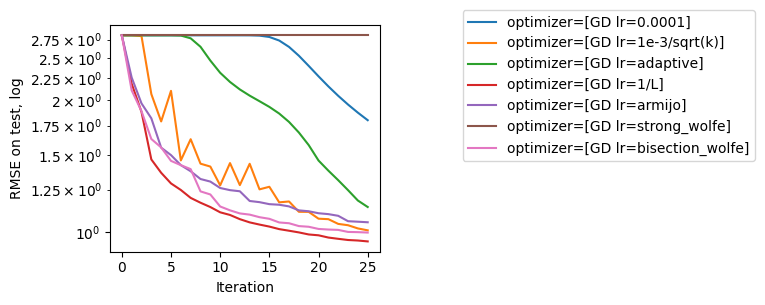
\includegraphics[width=\textwidth,keepaspectratio]{../data/gd.png}
       \caption[Gradient descent]{Gradient descent}\label{fig:gd}
     \end{figure}
   \end{frame}

   \begin{frame}
     \frametitle{Experiments. Heavy Ball}
     \begin{figure}[H]
       \centering
       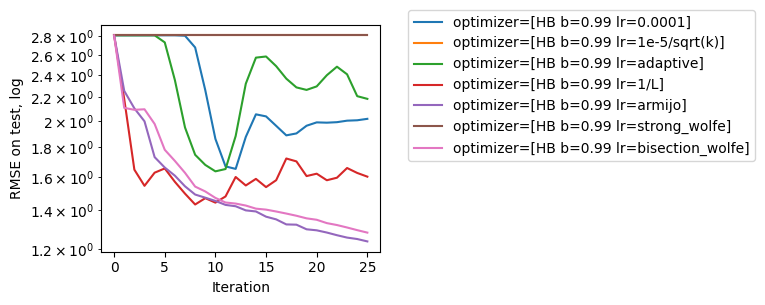
\includegraphics[width=\textwidth,keepaspectratio]{../data/hb.png}
       \caption[Heavy Ball]{Heavy Ball}\label{fig:hb}
     \end{figure}
   \end{frame}

   \begin{frame}
     \frametitle{Experiments. Nesterov}
     \begin{figure}[H]
       \centering
       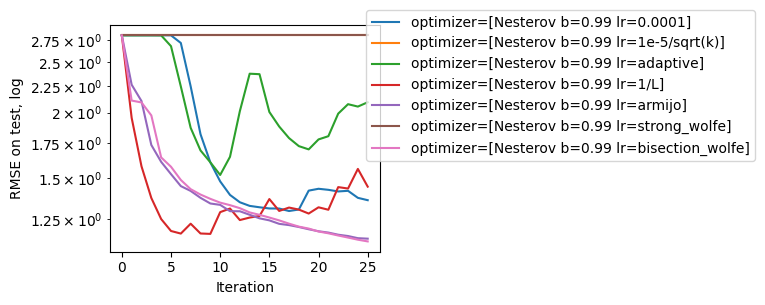
\includegraphics[width=\textwidth,keepaspectratio]{../data/Nesterov.png}
       \caption[Nesterov]{Nesterov}\label{fig:nesterov}
     \end{figure}
   \end{frame}

   \begin{frame}
     \frametitle{Experiments. RMSprop}
     \begin{figure}[H]
       \centering
       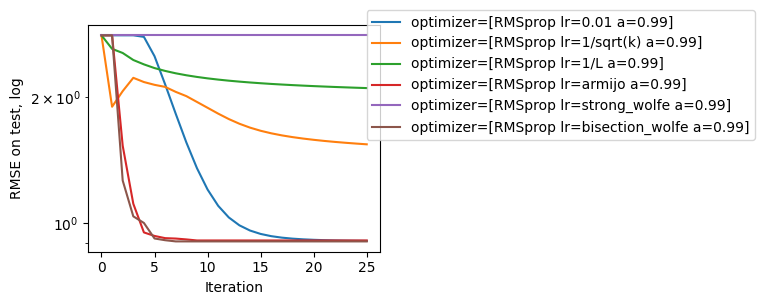
\includegraphics[width=\textwidth,keepaspectratio]{../data/rmsprop.png}
       \caption[RMSProp]{RMSprop}\label{fig:rmsprop}
     \end{figure}
   \end{frame}

   \begin{frame}
     \frametitle{Experiments. AdaGrad}
     \begin{figure}[H]
       \centering
       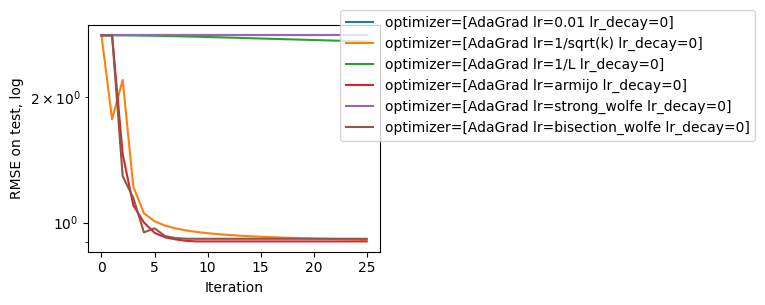
\includegraphics[width=\textwidth,keepaspectratio]{../data/adagrad.png}
       \caption[AdaGrad]{AdaGrad}\label{fig:adagrad}
     \end{figure}
   \end{frame}

   \begin{frame}
     \frametitle{Experiments. Adam}
     \begin{figure}[H]
       \centering
       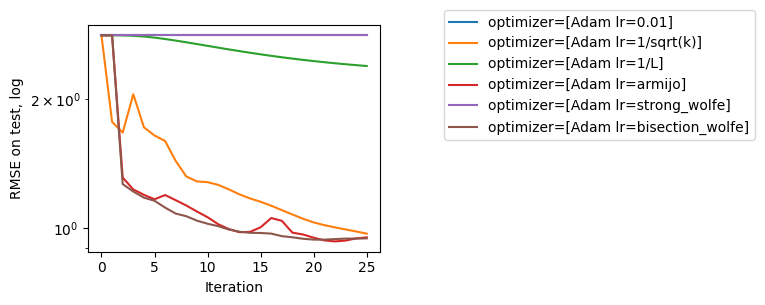
\includegraphics[width=\textwidth,keepaspectratio]{../data/adam.png}
       \caption[Adam]{Adam}\label{fig:adam}
     \end{figure}
   \end{frame}

   \begin{frame}
     \frametitle{Experiments. Comparison}
     \begin{figure}[H]
       \centering
       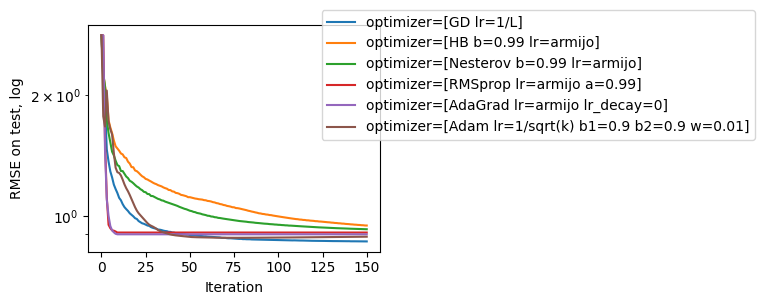
\includegraphics[width=\textwidth,keepaspectratio]{../data/comparison.png}
       \caption[Comparison]{Comparison}\label{fig:comparison}
     \end{figure}
   \end{frame}

   \begin{frame}
     Our best model with RMSE score 0.86 have the following parameters: $r=10$, GD optimizer with estimate 1/L strategy and $\lambda=2$
     \frametitle{Experiments. Best model}
     \begin{figure}[H]
       \centering
       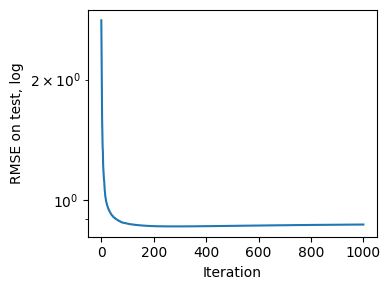
\includegraphics[keepaspectratio, scale=0.6]{../data/final.png}
       \caption[Best model]{Best model}\label{fig:best}
     \end{figure}
   \end{frame}

 \end{subsection}
\end{section}

\begin{section}{Vector Gradient Descent}
 \begin{frame}{Main idea}
   Instead of making update for entire $U$ or $V$ simultaneously, we can make updates row by row (column by column for $V$). The reasons are the following:
   \begin{itemize}
     \item The objective function becomes $f: \R^d \rightarrow \R$, so we can apply methods like BFGS
     \item There will be more updates, and such updates will be more diverse: we will use just updated values for new updates
   \end{itemize}
 \end{frame}
 \begin{frame}{Problem formulation}
   Therefore, the new problem with fixed $V$ becomes
   \begin{equation}\label{eq:vec_u}
     \min_{U^\top_i \in \R^r} \|W^\top_i \circ (X^\top_i - U^\top_i V)\|^2 + \lambda\|U^\top_i\|^2, \text{ }\forall i \in \{1,2,\ldots,m\}
   \end{equation}
   and the new problem with fixed $U$:
   \begin{equation}\label{eq:vec_v}
     \min_{V_j \in \R^r} \|W_j \circ (X_j - UV_j)\|^2  + \lambda\|V_j\|^2, \text{ }\forall j \in \{1,2,\ldots,n\}
   \end{equation}
 \end{frame}
 \begin{frame}{Gradients}
   Gradient of \Cref{eq:vec_u} is
   \begin{equation}\label{eq:vec_grads_u}
     \begin{aligned}
        & \frac{\partial (\|W^\top_i \circ (X^\top_i - U^\top_i V)\|^2 + \lambda\|U^\top_i\|^2)}{\partial U^\top_i} = \\
        & = -2 (W^\top_i \circ X^\top_i) V^T + 2 (W^\top_i \circ (U^\top_i V)) V^T + 2\lambda U^\top_i
     \end{aligned}
   \end{equation}
   and the gradient of \Cref{eq:vec_v}:
   \begin{equation}\label{eq:vec_grads_v}
     \begin{aligned}
        & \frac{\partial (\|W_j \circ (X_j - UV_j)\|^2  + \lambda\|V_j\|^2)}{\partial V_j} = \\ & = -2 U^T (W_j \circ X_j) + 2 U^T (W_j \circ (UV_j)) + 2\lambda V_j
     \end{aligned}
   \end{equation}
 \end{frame}
 \begin{frame}{Algorithm}
   \begin{algorithm}[H]
     \caption{Vector Gradient Descent}\label{algo:vec_grad}
     \begin{algorithmic}[0]
       \Require{$X, W \in \R^{m \times n}$ --- given initial and binary matrices,
         $U \in \R^{m \times r}, V \in \R^{r \times n}$ --- arbitrary matrices,
         $k_U$, $k_V$ --- small integers such that $\frac{m}{n} \approx \frac{k_U}{k_V}$}
       \State{}
       \State{$d \gets k_U + k_V $}
       \Repeat
       \For{$t = 0$ \textbf{to} $n+m-1$}
       \State{$r \gets t \textbf{ mod } d $}
       \If{$r < k_U$}
       \State{$i \gets k_U \cdot (t \textbf{ div } d) + r +1 $}
       \If{$i > m$}
       \State{\textbf{continue}}
       \EndIf{}
       \State{Update $U^\top_i$ using \Cref{eq:vec_grads_u}}
       \Else{}
     \end{algorithmic}
   \end{algorithm}
 \end{frame}


 \begin{frame}
   \begin{algorithm}[H]
     \renewcommand{\thealgorithm}{}

     \caption{Vector Gradient Descent. Continue}
     \begin{algorithmic}[0]
       \State{\ldots}
       \Repeat
       \For{$t = 0$ \textbf{to} $n+m-1$}
       \State{\ldots}
       \If{$i > m$}
       \State{\ldots}

       \Else{}
       \State{$j \gets k_V \cdot (t \textbf{ div } d) + r - k_U +1 $}
       \If{$j > n$}
       \State{\textbf{continue}}
       \EndIf{}
       \State{Update $V_j$ using \Cref{eq:vec_grads_v}}
       \EndIf{}
       \EndFor{}
       \Until{convergence}
       \State{}
       \State{\Return{$U,V$}}
     \end{algorithmic}
   \end{algorithm}
 \end{frame}

 \begin{frame}
   \frametitle{Experiments. Results}
   \begin{figure}[H]
     \centering
     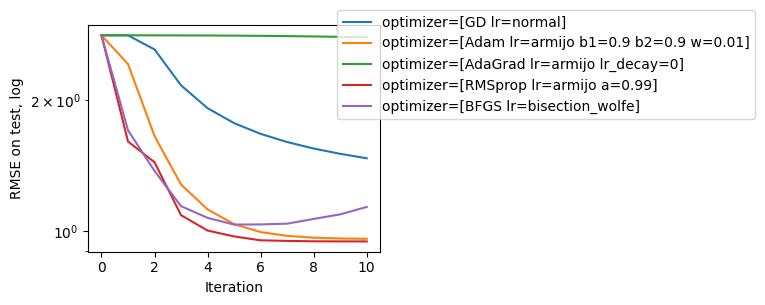
\includegraphics[width=\textwidth,keepaspectratio]{../data/vector_gd.png}
     \caption[Vector GD]{Vector Gradient Descent}\label{fig:vector_gd}
   \end{figure}
 \end{frame}
\end{section}

\begin{section}{NNMF}

 \begin{subsection}{Non-negative Matrix Factorization}

   \begin{frame}
     \frametitle{NNMF. Problem formulation}

     We want to solve initial problem (\ref{initial}), but with non-negativity constraints:
     \begin{equation}
       \min_{U \in \R^{m\times r}, V \in \R^{r\times n}} \|W \circ (X - UV)\|^2_F
     \end{equation}
     s.t. $U, V \geq 0$

     In order to solve such problem more easily, we need to derive multiplicative updates for $U$ and $V$.

   \end{frame}

   \begin{frame}
     \frametitle{MU updates}

     With the idea from \href{https://proceedings.neurips.cc/paper_files/paper/2000/file/f9d1152547c0bde01830b7e8bd60024c-Paper.pdf}{\underline{Lee and Seung paper}} we defined our MU updates in such way:

     \begin{equation}
       U \leftarrow U \circ \cfrac{((W \circ X) V^T)}{((W \circ (UV)) V^T + \epsilon)}
     \end{equation}

     \begin{equation}
       V \leftarrow V \circ \cfrac{(U^T (W \circ X))}{(U^T (W \circ (UV)) + \epsilon)}
     \end{equation}

   \end{frame}

 \end{subsection}

 \begin{frame}
   \frametitle{Experiments. Results}
   \begin{figure}[H]
     \centering
     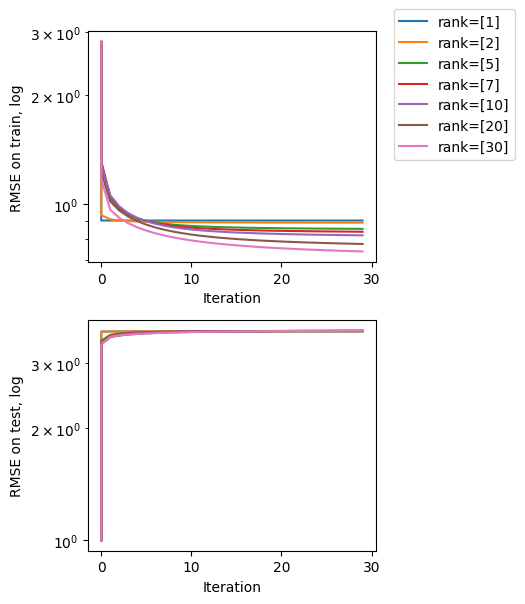
\includegraphics[keepaspectratio, scale=0.4]{../data/nnmf.png}
     \caption[NNMF]{NNMF}\label{fig:nnmf}
   \end{figure}
 \end{frame}

\end{section}

\begin{section}{Neural Network}

 \begin{subsection}{Structure}

   \begin{frame}
     \frametitle{Neural Network. Setup}

     As an alternative approach we decided to train simple neural network with such parameters:
     \begin{itemize}
       \item 4 layers ($23\times64, 64\times128, 128\times64, 64\times1$)
       \item ReLU as activation function after each layer
       \item MSELoss criterion
       \item Adam optimizer with $\alpha = 0.001$
       \item Early stopping (if on test set loss is not decreasing for 3 iterations)
       \item Maximum number of training epochs = 50
     \end{itemize}
   \end{frame}

   \begin{frame}
     \frametitle{Input/Output}
     As input to our model we decided to use:
     \begin{itemize}
       \item Min-max scaled `user\_id'
       \item Min-max scaled `movie\_id'
       \item One-hot encoded `genres' (we have 18 unique genres)
       \item Binary encoded `gender'
       \item Min-max scaled first two user features (`feature\_1' and `feature\_2`)
     \end{itemize}

     In output we have just one number - rating for specific pair of user and film.

     As a result we achieved average loss on test set 1.1
   \end{frame}

 \end{subsection}

\end{section}

\begin{section}{Overall Results}
 \begin{frame}{Overall Results}
   We tested several approaches: Gradient descent, Vector Gradient descent, Non-Negative Matrix Factorization and Neural Network.

   \begin{itemize}
     \item Both Neural Network and Vector Gradient descent showed their applicability for recommendation system task, however, they have been outperformed by other models
     \item NNMF is inapplicable for recommendation system task mostly because of the mask in the problem formulation. Mask makes NNMF to set almost all unknown values to 1, which is very bad decision
     \item It happens to be that Gradient descent method showed the best overall performance (both in terms of time and score). We were able to achieved RMSE score 0.86 on test data
   \end{itemize}

 \end{frame}

 \begin{frame}{Conclusions}
   \huge
   \begin{equation*}
     \textbf{Thanks!}

   \end{equation*}


 \end{frame}

\end{section}
\end{document}
